
\subsubsection{模型建立}

针对问题三，本节将建立基于二分搜索的临界填充率定位模型。具体过程如下。

\textbf{步骤1：二分搜索框架}

设$f(N)$为颗粒数为$N$时的真实导通概率（未知），$\hat{f}_M(N)$为基于$M$次蒙特卡洛试验的概率估计值。二分搜索的伪代码如下：

初始区间$[N_L, N_H] = [5, 80]$，终止条件$N_H - N_L \leq 1$。每轮迭代：
\begin{equation}
N_{\text{mid}} = \left\lfloor \frac{N_L + N_H}{2} \right\rfloor
\end{equation}
计算$\hat{f}_M(N_{\text{mid}})$：
\begin{equation}
\hat{f}_M(N_{\text{mid}}) = \frac{1}{M} \sum_{m=1}^{M} X_m(N_{\text{mid}})
\end{equation}
其中$X_m(N_{\text{mid}}) \in \{0, 1\}$为第$m$次试验的导通状态，$M=200$。

若$\hat{f}_M(N_{\text{mid}}) \geq 0.90$，则$N_H \leftarrow N_{\text{mid}}$；否则$N_L \leftarrow N_{\text{mid}} + 1$。

\textbf{步骤2：大样本验证}

二分搜索收敛后得到估计的最小颗粒数$N_{\min}$，对应的填充率为：
\begin{equation}
\phi_{\min} = \frac{N_{\min} \cdot V_A}{V_{\text{total}}}
\end{equation}

为确保结果的统计可靠性，对$N_{\min}$进行更大规模的蒙特卡洛验证（$M_v = 500$次）：
\begin{equation}
\hat{P}_c^{\text{verify}} = \frac{1}{M_v} \sum_{m=1}^{M_v} X_m(N_{\min})
\end{equation}
计算95\%置信区间：
\begin{equation}
\text{CI}_{95\%} = \hat{P}_c^{\text{verify}} \pm 1.96 \cdot \sqrt{\frac{\hat{P}_c^{\text{verify}}(1 - \hat{P}_c^{\text{verify}})}{M_v}}
\end{equation}

\textbf{步骤3：精细概率曲线}

在$N_{\min}$附近以步长1生成精细的概率-颗粒数曲线，观察渗透阈值附近的概率跃迁行为，验证结果的合理性。

\subsubsection{模型求解}

基于上述模型，本节执行二分搜索并分析结果。二分搜索的收敛过程如表\ref{tab:二分过程}所示。

\begin{longtable}{>{\centering\arraybackslash}p{0.10\textwidth}>{\centering\arraybackslash}p{0.14\textwidth}>{\centering\arraybackslash}p{0.14\textwidth}>{\centering\arraybackslash}p{0.14\textwidth}>{\centering\arraybackslash}p{0.14\textwidth}}
  \caption{二分搜索收敛过程}
  \label{tab:二分过程} \\
  \toprule
  迭代 & 下界N & 上界N & 中点N & 导通概率 \\
  \midrule
  \endfirsthead
  \caption{二分搜索收敛过程（续）} \\
  \toprule
  迭代 & 下界N & 上界N & 中点N & 导通概率 \\
  \midrule
  \endhead
  \bottomrule
  \endfoot
  1 & 5 & 80 & 42 & 0.9200 \\
  2 & 5 & 42 & 23 & 0.7400 \\
  3 & 24 & 42 & 33 & 0.8350 \\
  4 & 34 & 42 & 38 & 0.8650 \\
  5 & 39 & 42 & 40 & 0.9200 \\
  6 & 39 & 40 & 39 & 0.9150 \\
\end{longtable}

由表\ref{tab:二分过程}可知，二分搜索仅用6轮即收敛至$N_{\min}=39$。第1轮即发现N=42时概率已达92.00\%，证实了渗透阈值远低于0.50\%的初步判断。

大样本验证结果：500次试验中导通453次，$\hat{P}_c^{\text{verify}} = 0.9060 \pm 0.0131$，95\%置信区间为$[0.8804, 0.9316]$。最小填充率$\phi_{\min} = 39 \times 1.4137 \times 10^7 / 10^{12} = 0.0551\%$。

\begin{figure}[ht]
  \centering
  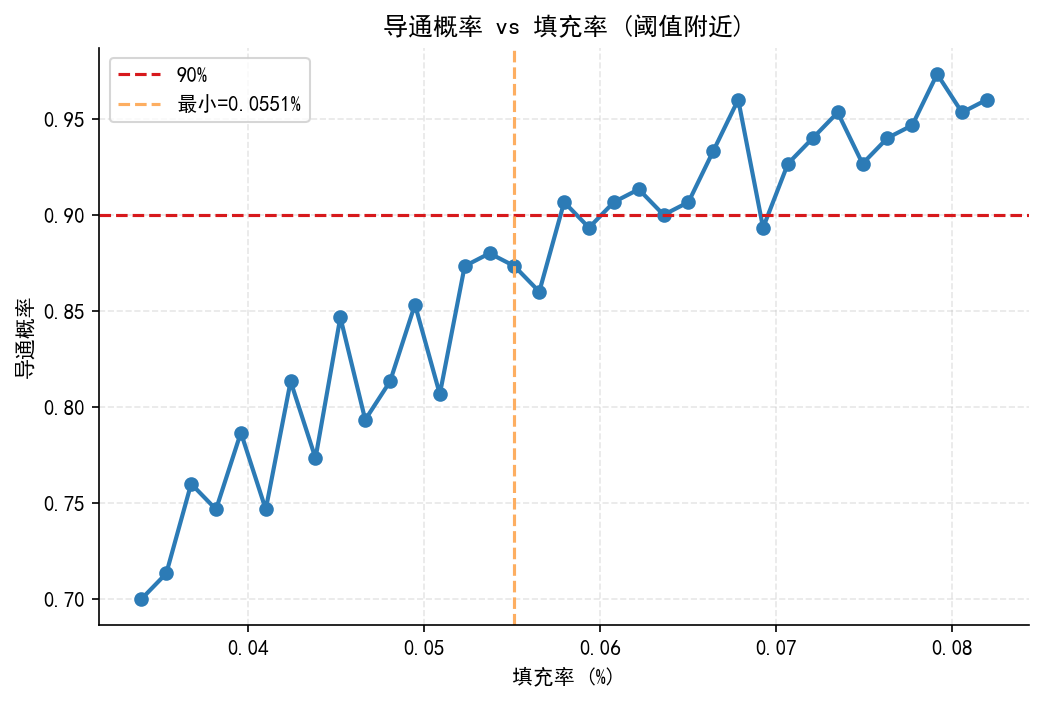
\includegraphics[width=0.8\textwidth]{../求解/问题三/图片/导通概率vs填充率曲线_精细.png}
  \caption{渗透阈值附近的精细概率曲线}
  \label{fig:q3_prob}
\end{figure}

\begin{figure}[ht]
  \centering
  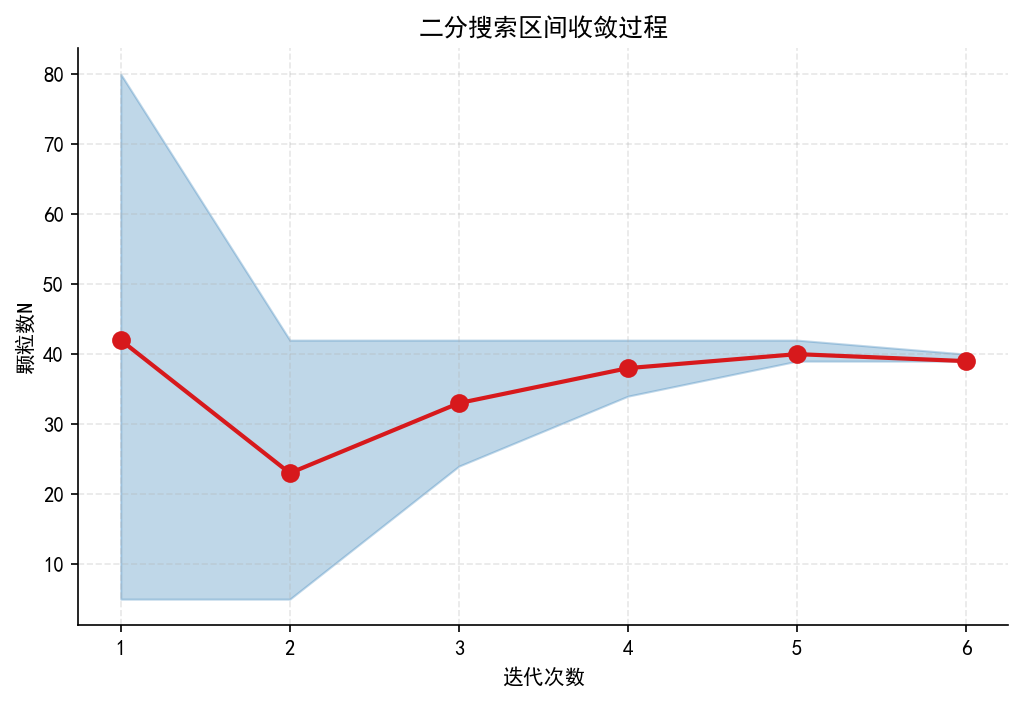
\includegraphics[width=0.8\textwidth]{../求解/问题三/图片/二分搜索收敛图.png}
  \caption{二分搜索区间收敛过程}
  \label{fig:q3_search}
\end{figure}

附件3的535个颗粒配置经判定为导通状态，填充率0.7563\%远高于临界值0.0551\%，符合预期。

如图\ref{fig:q3_prob}所示，导通概率在填充率0.03\%至0.06\%之间呈现典型的渗透相变行为——从约70\%快速跃升至90\%以上。这一超低渗透阈值源于金属A圆柱体极高的长径比（83:1），与理论预测$\phi_c \propto 1/\alpha$一致。综上所述，问题三确定了使导通概率不低于90\%的最小填充率为0.0551\%，对应39个金属A圆柱体。
